\documentclass[12pt,oneside]{sotsuken_paper}

% タイトル
\title{1軸レーザー距離センサを用いたQudad Rotorの周辺認識についての研究}
\author{織田隆誠・木村俊介・村田涼真}

\begin{document}
% 行間
\setlength{\baselineskip}{9truemm}

%文字間
\kanjiskip=.53zw plus 3pt minus 3pt
\xkanjiskip=.53zw plus 3pt minus 3pt

% 目次
\tableofcontents
%\newpage

% 本文

\chapter{序論}
\section{研究の背景}
東日本大震災時に,福島第一原子力発電所の原子炉内でメルトダウンが起こりその後,原発内の状況把握や上空からの映像を撮影可能であったのも無人ロボットのおかげである.\\室内の撮影にはクローラーを用いて陸を走行するタイプの無人ロボット(Uninhabited Ground Vehicle:UGV)が活躍し,上空からの撮影が可能であったのは,無人航空機(Uninhabited Aerial Vehicle:UAV)のおかげである.以前からUAVなどの研究はされてはいたが,当時はまだUGVやUAVが一般的ではなく、知名度は低かった、しかし福島第一原子力発電所の事故が起きた時に、東京電力の呼びかけでいくつかの研究チームや企業が協力し状況把握,撮影等が可能になった.その後全国でUGVやUAVの研究,開発が盛んに行われるようになった.


我々の研究室ではUAVについて研究を行っている.
軍事目的では早い時期から実用化されており,民間でも農薬散布などの目的に実用化されている.
そもそもUAVとは,人が搭乗せずに遠隔操作や自動制御をなどを用いて飛行を行う無人航空機の総称である\cite{hirokawa2007}.


UAVには様々な形状,大きさなどが存在するが,図\ref{fig:1}に示すようなマルチコプターの登場により研究開発が活性化してきており,様々な分野での活躍が期待されている.我々の研究では4枚のプロペラを使い飛行を行う「Quad Rotor」をついて研究を行っている.

\begin{figure}[H]
\begin{center}
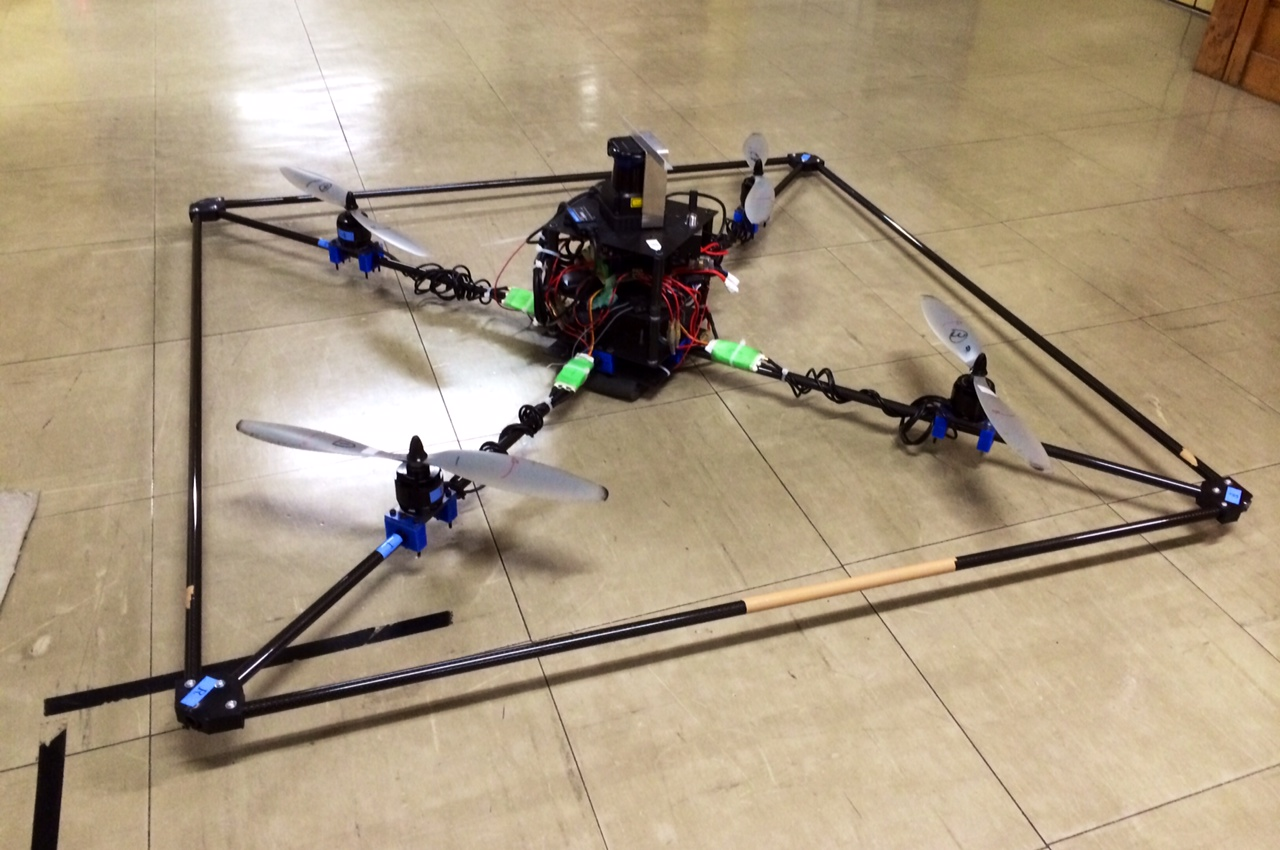
\includegraphics[width=120mm]{img/1.jpg}
\end{center}
\caption{研究用Quad Rotor}
\label{fig:1}
\end{figure}

\section{UAVの活躍}
従来,UAVは軍事目的による使用が盛んである.
図\ref{fig:hara}に示すようなUAVで危険な敵地への偵察や爆撃,友軍への支援物資の運搬など様々な用途で使われてきた.
近年では一般の企業や個人の趣味などでUAVを利用するケースが増加している傾向にある.
図\ref{fig:multi}に示すUAVは空から写真,映像の撮影を行うUAVで機体の下にカメラが搭載可能である.そういった装備が簡単に搭載できることから,ホビーとしてUAVの操作を楽しむ人が増えてきている.
警備会社などではUAVを使った防犯監視システムへの利用.
大手通販会社のAmazonでは,図\ref{fig:Ama}に示すようなUAVで2015年度から一部地域でのUAVによる荷物の配送実験が行われている.
GoogleではGoogleMapの地図作成など様々な用途でが使用されていることが分かる.


\begin{figure}[H]
\begin{center}
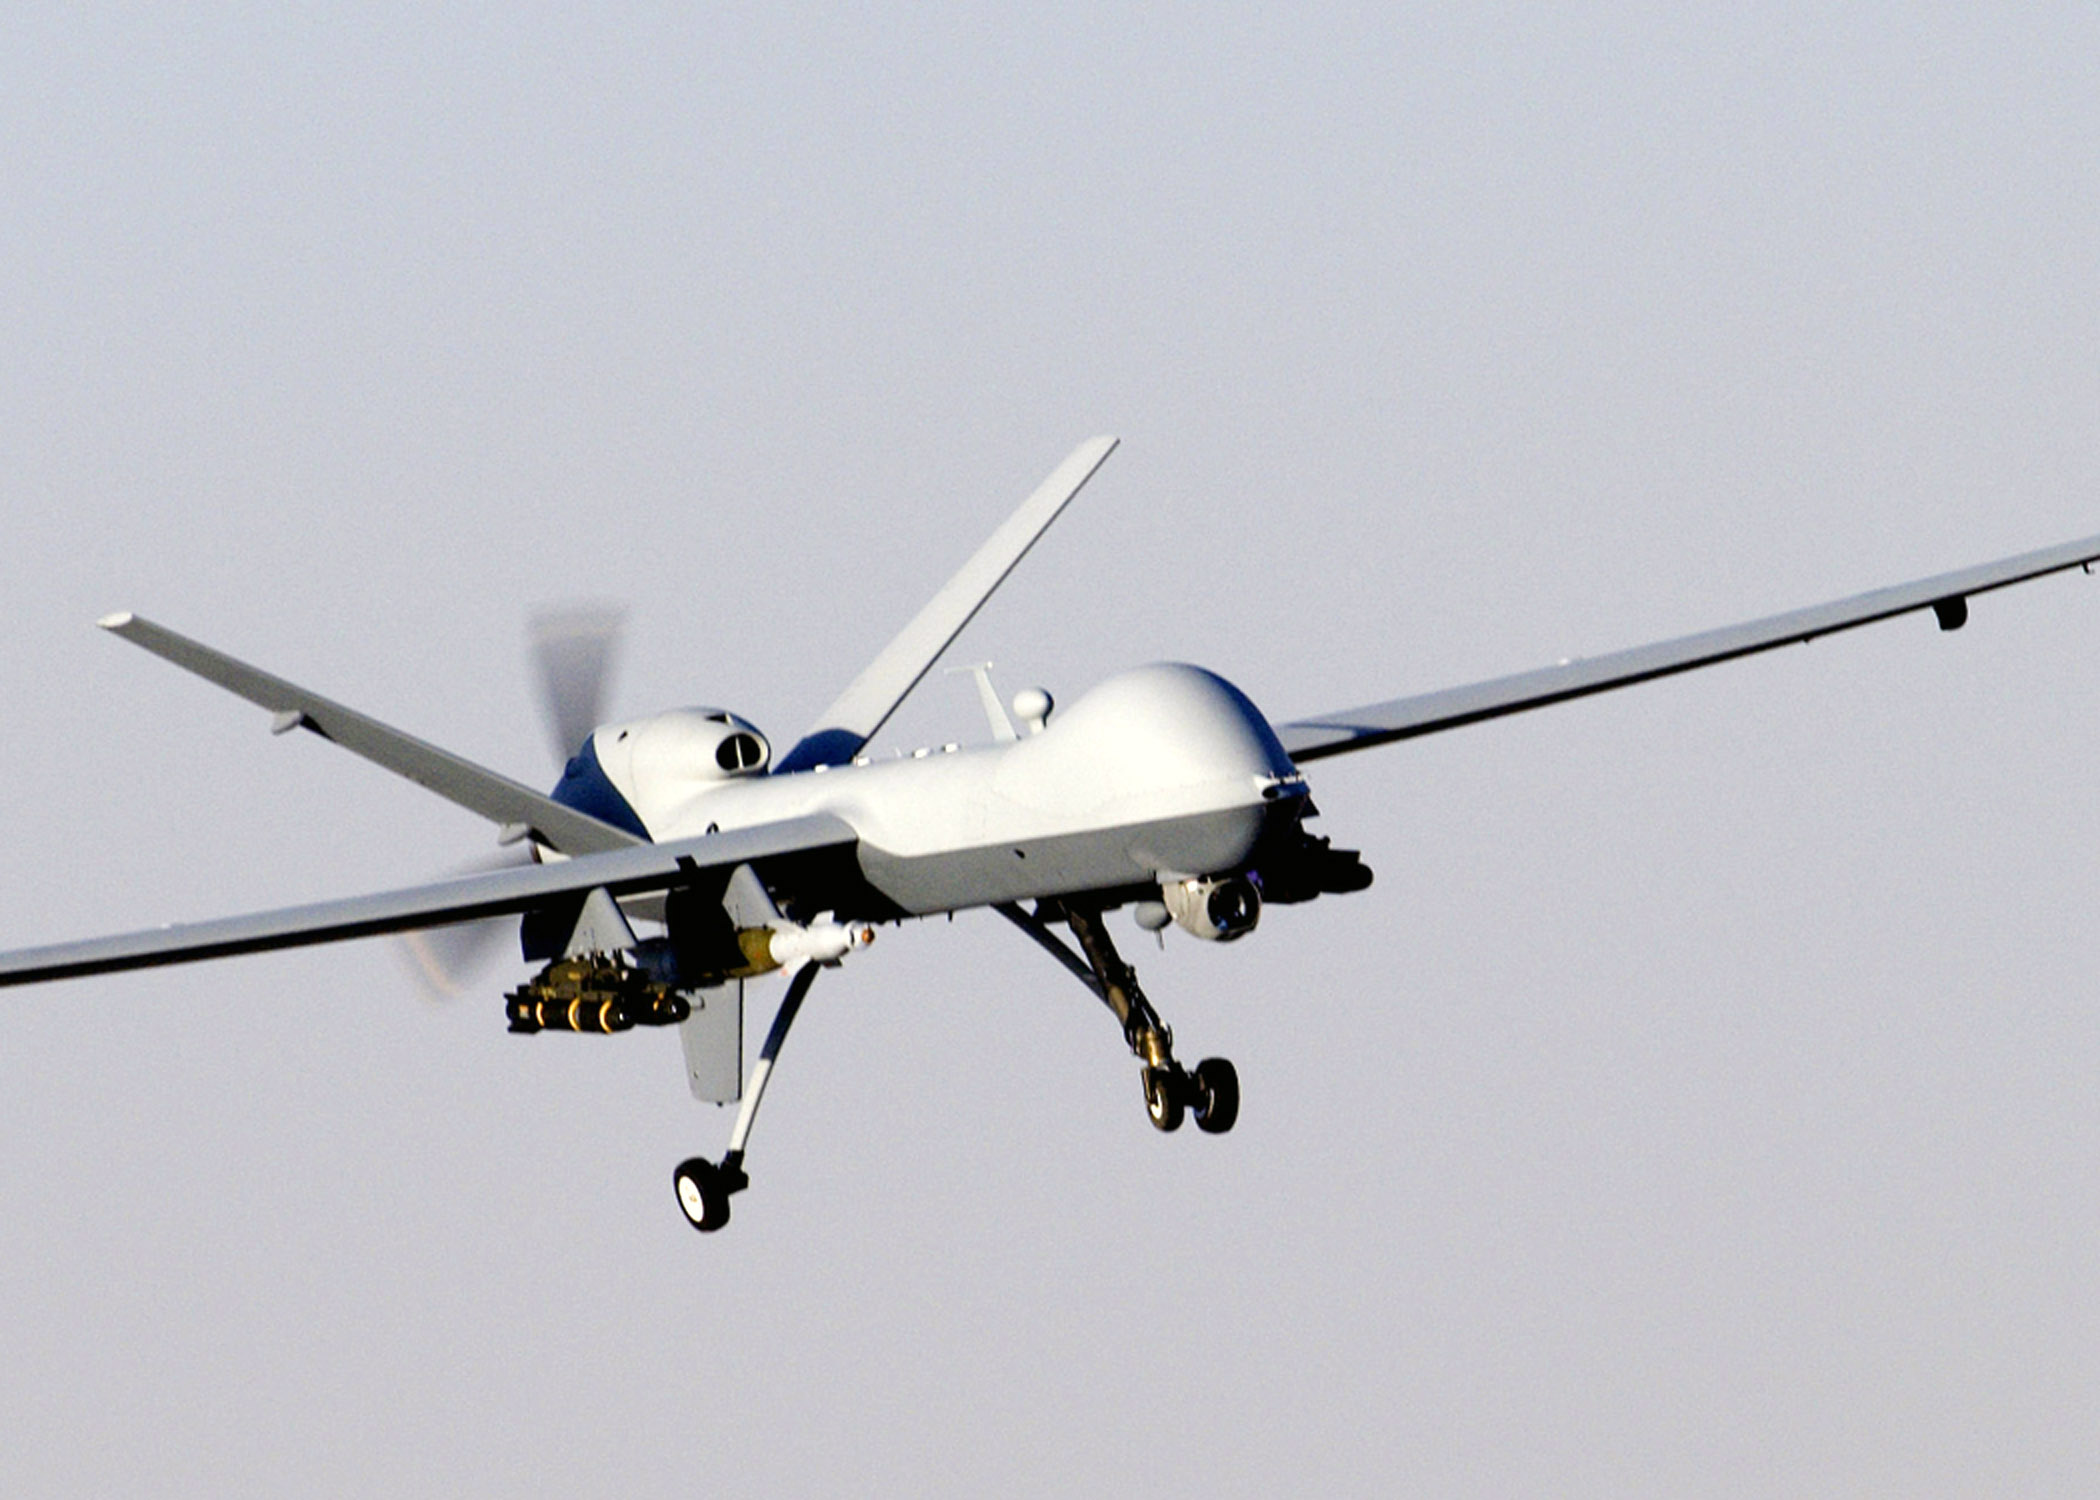
\includegraphics[width=120mm]{img/hara.jpg}
\end{center}
\caption{アメリカ空軍で使用されるMQ-9 Reaper}
\label{fig:hara}
\end{figure}

\begin{figure}[H]
\begin{center}
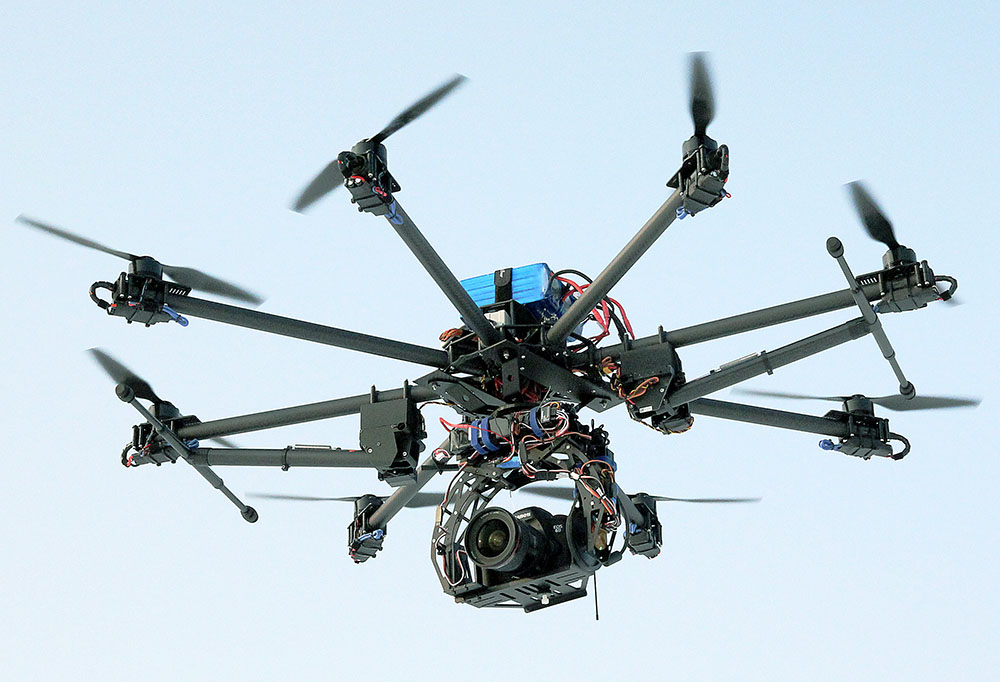
\includegraphics[width=120mm]{img/multi.jpg}
\end{center}
\caption{空撮用UAV}
\label{fig:multi}
\end{figure}

\begin{figure}[H]
\begin{center}
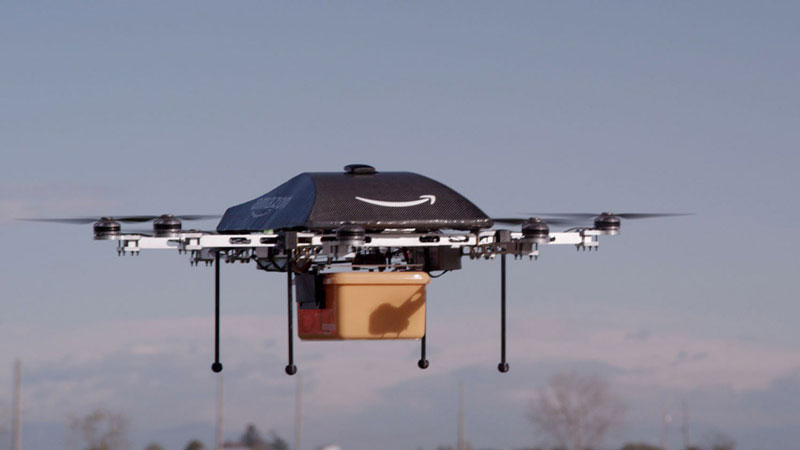
\includegraphics[width=120mm]{img/Ama.jpg}
\end{center}
\caption{Amazonで使用されるUAV}
\label{fig:Ama}
\end{figure}

\section{UAVの運用条件}
多くの事に利用できるUAVであるが,利用目的が増えるとともに装備する付属機器や電子部品などの量が増加し,重量が非常に重くなってしまう.
重量の増加に伴い機体自体の大きさが大型化してしまうと室内や複雑に入り組んだエリアの運用では大きな障害となり,運用が難しくなってしまう.
そこで我々は,汎用性の高いUAVとは何かについて考えてみた.
室内での運用を考え,一般住宅の窓枠を参考にし,機体の大きさは一辺が30cmの正方形、比較的重量が重くなると考えられるセンサは約100g程度が良いのではないかと考える.




\section{研究の目的}
UAVの活用の場として偵察,監視,空撮,地図作成,運搬等が考えられそれらは,UAVに適当なセンサを搭載し制御できることが求められる.レーザスキャナを搭載するためには,その重量を運搬可能な機体が必要である.一般の空撮に比べ地図作成の場合は比較的大型の機体を用いる必要がある.理由としては,センサの重量,その他付属品が一般の空撮に比べ多いからである.仮に地図を作成しなければならない場所が屋内だとすると,屋外では図\ref{fig:hikou1}に示すように飛行可能だが,同じ大きさの機体では図\ref{fig:hikou2}に示すように飛行不可能になる,必然的にUAVの大きさの制限を受け,小型化を追求する事になる.このUAVの小型化という課題は今後UAVが活躍していく上で重要な項目である.
そこで筆者らはUAVに搭載するセンサの中で特に重要で重量が大きい,スキャン式レーザ距離計を,小型UAVに対応させるため軽量化した一軸レーザ距離計の試作を試みた.
今回はセンサ内のスキャン機構の機能を完全に停止させ,一軸化したと想定し実験を行い,有効性を確かめる.



\begin{figure}[H]
\begin{center}
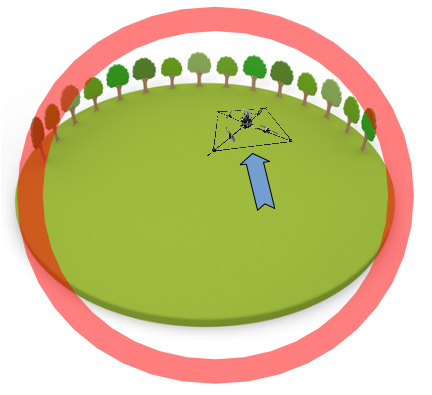
\includegraphics[width=90mm]{img/hikou1.png}
\end{center}
\caption{飛行可能状況}
\label{fig:hikou1}
\end{figure}

\begin{figure}[H]
\begin{center}
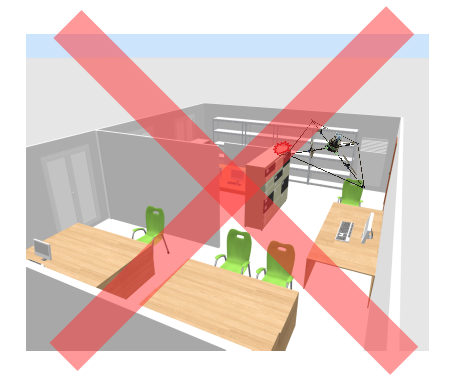
\includegraphics[width=90mm]{img/hikou2.png}
\end{center}
\caption{飛行不可能な状況}
\label{fig:hikou2}
\end{figure}


\section{論文の構成}
この論文では以下のように構成されている.
1章では,我々の研究目的やUAVの活用,運用について考察したものである.


2章では,各社のレーザセンサの調査,それの問題点そして,今回実験で使用するセンサの改良,利用方法について研究したものである.


3章では,Quad Rotorについての基本的な知識,構造,実験で使用したQuad Rotorについてと各種センサ類の接続方法について記されている.


4章では,今回行った1軸センサを利用した周辺認識実験の概要と方法を説明し,結果と考察を報告したものである.


5章では,前章で行った実験の結果と考察を元に本実験の結言を記す.


6章では,本研究において大きな力となった関係者各員に謝辞を記す.
\chapter{レーザセンサについて}UAVを安全かつ効率的に自律化し運用するためには,周辺環境を読み取り現在地の状況を正しく把握する必要がある.\\
そのため,UAVの自動制御においてレーザセンサは非常に重要なパーツであり,必要不可欠である.\\
しかし,高性能なものはそれに伴い重量の大きいパーツのひとつになってしまうと考えられる.\\


\section{各社レーザセンサの調査}センサの軽量化を図るに際して,我々は現在各社で販売されている測域センサについて調査を行った.その結果,図\ref{fig:re-za}のようにUAVに搭載するものとしては各社とも重量が非常に重く,小型機体への搭載は非現実的であり運用は難しいことが判った.\\
 そこで,我々は測域センサから機能を制限した一軸レーザセンサの使用を考えた.
前方向にしか計測できない一軸レーザセンサだがその分軽量化できると考えた.
だが,我々の予想に反し,図\ref{fig:re-za2}から分かるとおり,一軸レーザセンサも比較的重量が重いものが多かった.\\
 小型で軽量な製品もあったものの,計測距離が短くこちらもUAVに搭載し,自律飛行に用いるものとしては不十分な性能だった.

\begin{figure}[H]
\begin{center}
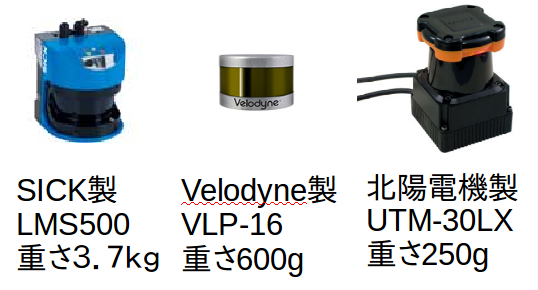
\includegraphics[width=120mm]{img/re-za.png}
\end{center}
\caption{各社レーザセンサの計測距離と重量}
\label{fig:re-za}
\end{figure}

\begin{figure}[H]
\begin{center}
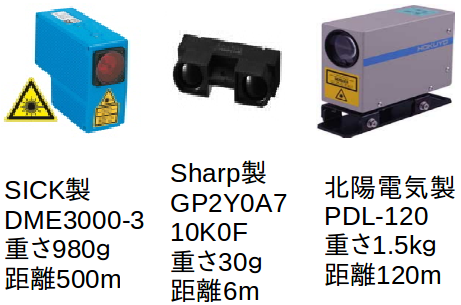
\includegraphics[width=120mm]{img/ichizikure-za.png}
\end{center}
\caption{各社一軸レーザセンサの距離と重量}
\label{fig:re-za2}
\end{figure}


\section{スキュン式レーザ距離計の一軸レーザ距離センサへの改良}
UAVによる周辺状況の取得には,スキャン式レーザ距離計を用いるのが一般的であるが,UAVの軽量化を目標としたときに,スキャン式レーザ距離計の重量は無視できないものとなる.\\
そこで,スキャン式レーザ距離計の信号処理系と光学系を流用し,大きな重量を要するスキャン機構を取り除くことで実現することとした.

\section{実験で使用するセンサ}
本研究では北陽電機製「UTM-30LX」を使用する.
実際に軽量化を行った際,一軸化した測域センサはUAVにおいて有用的に運用できるか検証を行う.

\begin{figure}[H]
\begin{center}
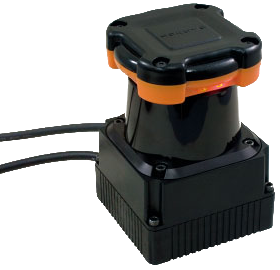
\includegraphics[width=50mm]{img/2.png}
\end{center}
\caption{使用した一軸レーザセンサ}
\label{fig:2}
\end{figure}

\section{センサの軽量化}
測域センサは広範囲のエリアを計測するため、内部にセンサを反射させる回転ミラーが搭載されている.
このミラーと回転に必要なモーターを外す事,つまり測域センサを一軸レーザー化する(図\ref{fig:kairyou})ことによってセンサは約100gほどの軽量化ができると考えた.

\begin{figure}[H]
\begin{center}
\includegraphics[width=100mm]{img/kairyou.png}
\end{center}
\caption{センサの機能を一部取り除く}
\label{fig:kairyou}
\end{figure}

しかし,センサは連続使用し続けると本体が熱を持ち始め図\ref{fig:gurahu}から見て取れるように,計測距離に誤差が出始める.

\begin{figure}[H]
\begin{center}
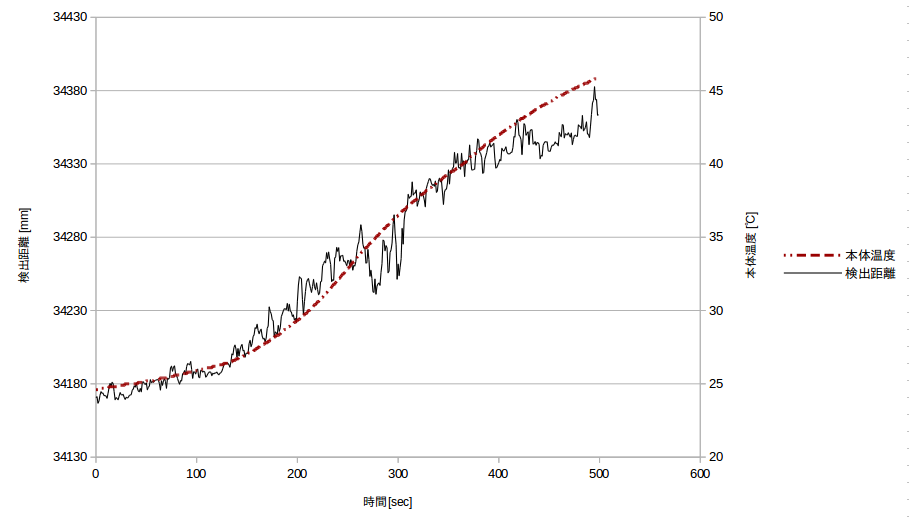
\includegraphics[width=160mm]{img/gurahu.png}
\end{center}
\caption{レーザセンサ本体の熱と検出距離の関係}
\label{fig:gurahu}
\end{figure}

本来,測域センサの場合,レーザが回転するたびに内部に搭載された基準板を検出し,誤差の修正を行う.
しかし一軸レーザ化することによってこの機能は使用することができなくなってしまい,連続で運用した場合,致命的な動作不良になり得る可能性がある.そこで我々は以下の対策を講じた.

\section{マルチエコー機能を使用した熱による誤差への対策}
「UTM-30LX」には「マルチエコー機能」という機能が搭載されている.
この機能は,雨や本体の汚れ,ホコリなどが測定方向に入り込み,正確な距離を計測できなくなるのを防ぐための機能である\cite{si2014}.
通常のセンサは物体から一つのエコーを処理して物体までの距離を計測するが図\ref{fig:marutieko2}に示すようにレーザには幅が存在するため,複数の物体から複数のエコーを受け取ることが可能であり,複数のエコーからそれぞれに距離を出力することができる機能である.

\begin{figure}[H]
\begin{center}
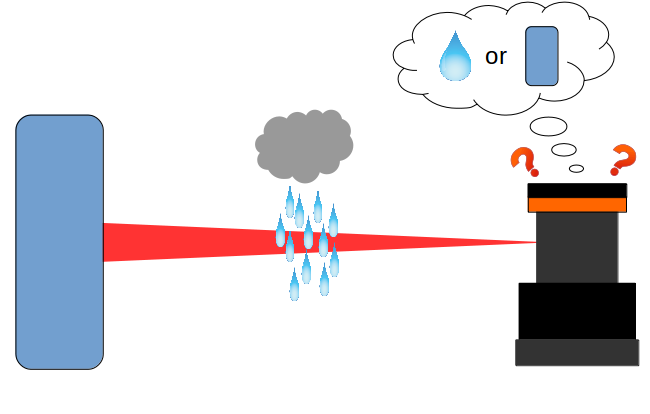
\includegraphics[width=80mm]{img/marutieko2.png}
\end{center}
\caption{複数の物体距離を計測できるマルチエコー機能}
\label{fig:marutieko2}
\end{figure}

この機能を使い,本体の正面半分を一定距離においた板で覆い隠し,基準板として使う手法を考案した.
図\ref{fig:sensa3}のように計測したい距離と基準板を同じレーザーで測り,基準板のズレを計測結果にフィードバックする仕組みである.

\begin{figure}[H]
\begin{center}
\includegraphics[width=80mm]{img/sensa1.png}
\end{center}
%\caption{計測距離の誤差修正}
\label{fig:sensa1}
\end{figure}

\begin{figure}[H]
\begin{center}
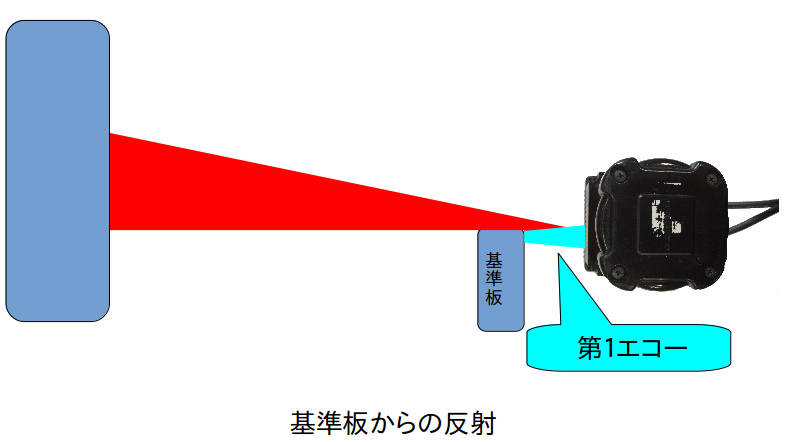
\includegraphics[width=80mm]{img/sensa2.png}
\end{center}
%\caption{計測距離の誤差修正}
\label{fig:sensa2}
\end{figure}

\begin{figure}[H]
\begin{center}
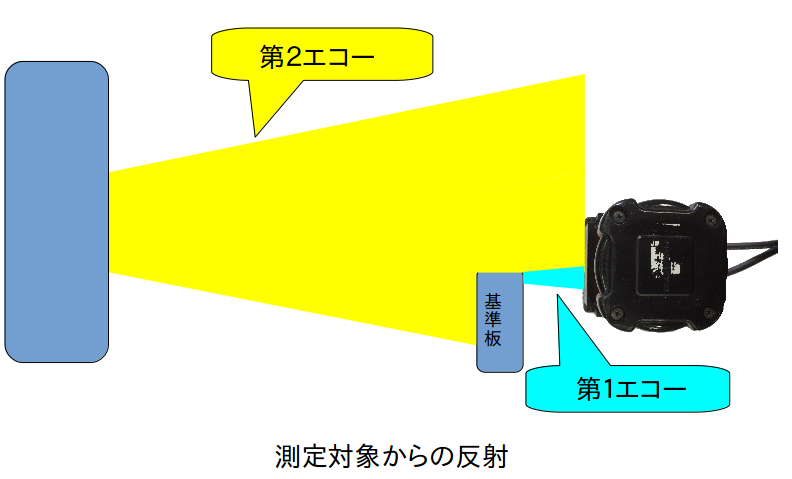
\includegraphics[width=80mm]{img/sensa3.png}
\end{center}
\caption{計測距離の誤差修正}
\label{fig:sensa3}
\end{figure}

\section{改良後のセンサの運用法}
しかし,先述の通り,測域センサを一軸化することによって広範囲のスキャンは不可能になった.
よって,図\ref{fig:unnyou}のように,センサを載せた機体を直接回転させる事によりこの欠点を補うこととする.

\begin{figure}[H]
\begin{center}
\includegraphics[width=80mm]{img/unnyou.png}
\end{center}
\caption{本体を回転させ地形をスキャンする}
\label{fig:unnyou}
\end{figure}


\begin{figure}[H]
\begin{center}
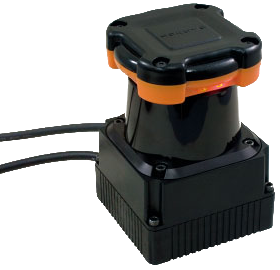
\includegraphics[width=50mm]{img/2.png}
\end{center}
\caption{使用した一軸レーザセンサ}
\label{fig:2}
\end{figure}

\chapter{Quad Rotorについて}多くのプロペラを使用する機体は図\ref{fig:heri}のよう翼の角度を調整するフラッピングや,フェザリングなどの複雑な翼制御を行う必要があり,専門知識のない人物にとって操縦や製作は非常に難しい物であった\cite{sibata2003}.
Quad Rotorとはプロペラを使用するUAVの形状の一種であるが.四枚の固定プロペラを制御することで上記の操作を行うことができ,GPSのような位置安定装置を利用することで,専門知識がなくても自由度の高い動きで,UAVを飛ばすことが容易にできる構造になっている.
UAVの形状の中では比較的知名度があり,個人の趣味や一般企業などでも高い頻度で使用されている.

\begin{figure}[H]
\begin{center}
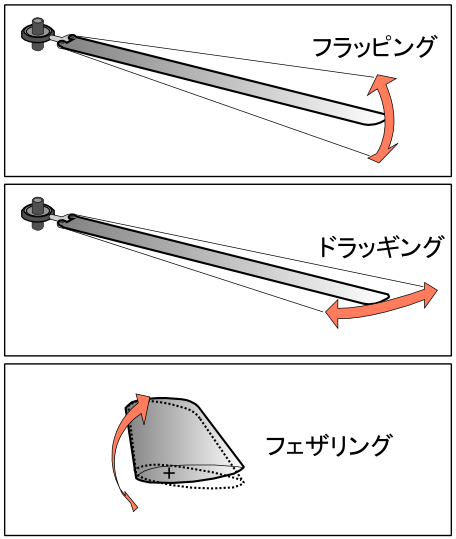
\includegraphics[width=50mm]{img/heri.png}
\end{center}
\caption{翼の動き}
\label{fig:heri}
\end{figure}

\section{実験で使用するQuado Rotor}我々の研究室では毎年新しいQuad Rotorの作成を行っており、図\ref{fig:1}は今年度に作成し,実験で使用したQuad Rotorである.

\begin{figure}[H]
\begin{center}
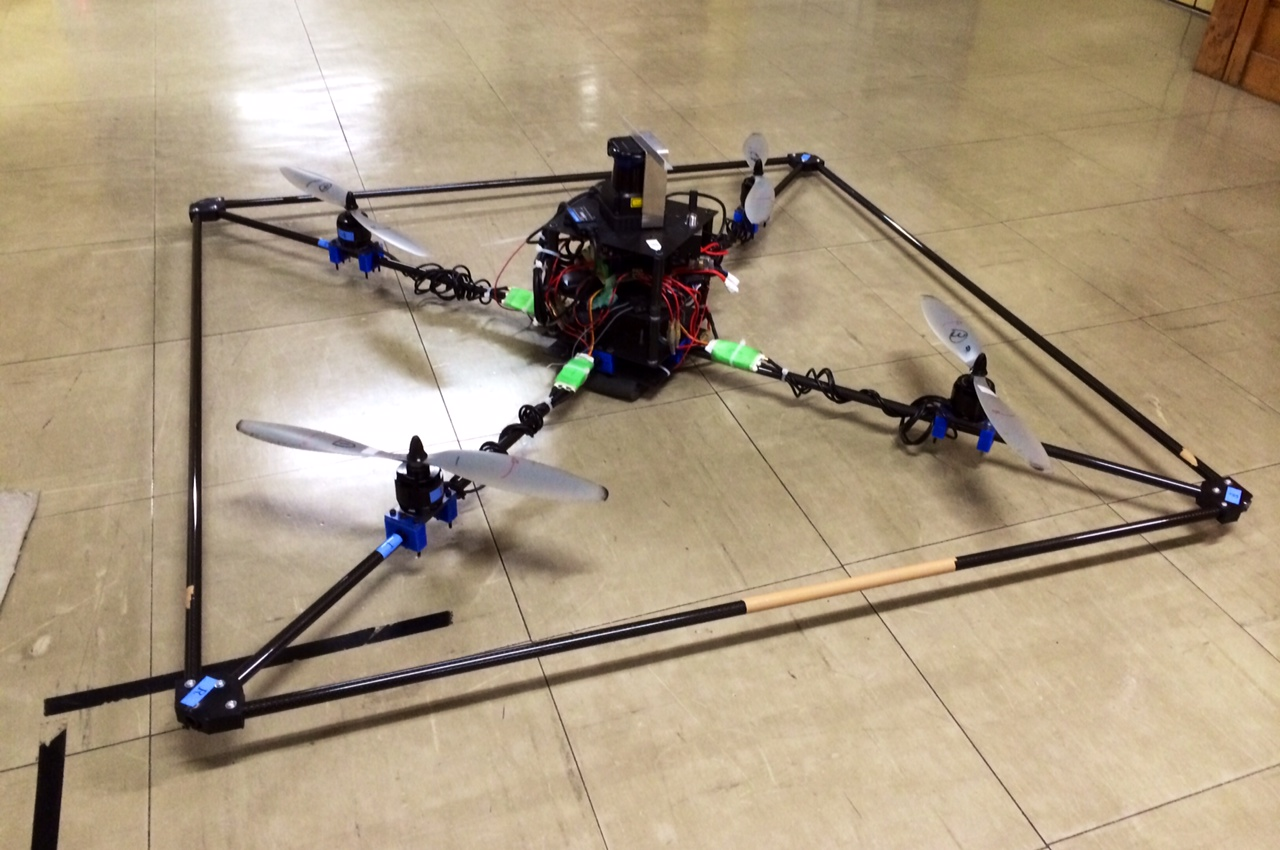
\includegraphics[width=130mm]{img/1.jpg}
\end{center}
\caption{実験で使用したQuad Rotor}
\label{fig:1}
\end{figure}

Quad Rotorの大きさは1辺950mmの正方形の形をしている.本年度は軽量化のためフレームや基板を取り付けるプレートの素材を従来使用していたアルミフレームからカーボンフレームに変更した.変更したことにより約1.5kgの減量に成功した.

\begin{figure}[H]
\begin{center}
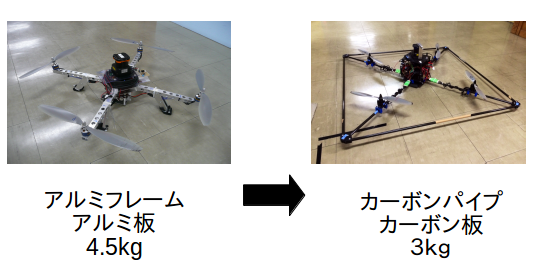
\includegraphics[width=140mm]{img/omosa.png}
\end{center}
\caption{フレーム類をアルミからカーボンに変更した機体}
\label{fig:omosa.jpg}
\end{figure}

モータはT-Moter社製のU20に変更し,昨年使用したものと同じプロペラを使用した状態で推力が前のモータに比べ2倍になった.

\begin{figure}[H]
\begin{center}
\includegraphics[width=150mm]{img/mo-ta.png}
\end{center}
\caption{モーターの変更}
\label{fig:mo-ta}
\end{figure}

バッテリーは大容量のものに変更し連続してホバリングを続けれる時間が5分から約10分に伸びた.
\begin{figure}[H]
\begin{center}
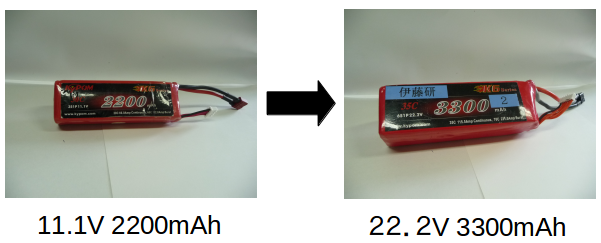
\includegraphics[width=140mm]{img/denchi.png}
\end{center}
\caption{バッテリーの変更}
\label{fig:denchi}
\end{figure}

\section{搭載してる各種センサーの接続方法}
以下からUAVに搭載されているコントローラ受信機,APM,モータドライバとモータの接続,GPS,高度センサの接続について記載し,その配線図を記載する.
必ずバッテリーを取り外した状態で行う事に注意しなければならない.\\ 
1)APM,コントローラー受信機の接続\\
電源ケーブルをCPU基板に差し込みもう一方をコントローラー受信機B番ピンを図\ref{fig:setuzoku1}のようにに差し込む\\

\begin{figure}[H]
\begin{center}
\includegraphics[width=140mm]{img/setuzoku1.png}
\end{center}
\caption{コントローラー受信機へ電源の供給}
\label{fig:setuzoku1}
\end{figure}

赤,黒色両側2ピンのメス端子を隣の6番ピンに図\ref{fig:setuzoku2}のように取り付け,もう片方をAPM本体INPUTS側7番ピン上から1,2ピンに赤,黒の順に差し込む.\\

\begin{figure}[H]
\begin{center}
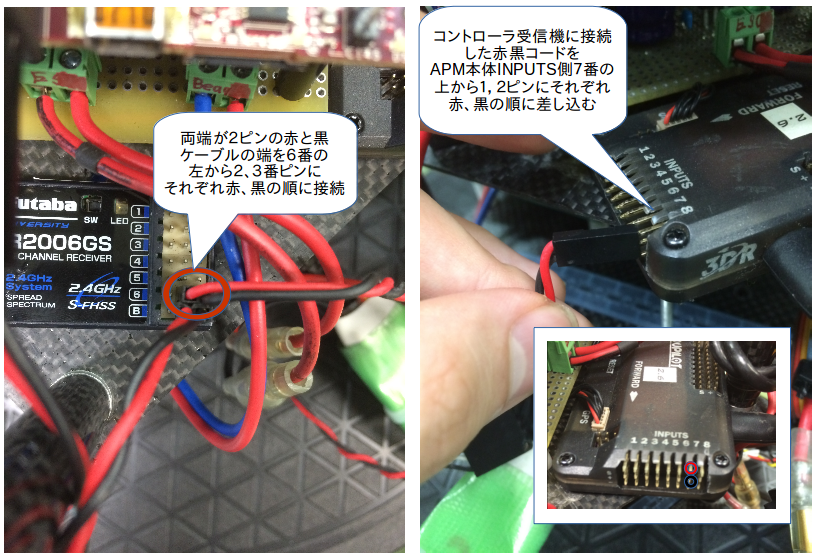
\includegraphics[width=140mm]{img/setuzoku2.png}
\end{center}
\caption{APMへ電源の供給}
\label{fig:setuzoku2}
\end{figure}

コントローラ受信機,1,2,3,4,5,6番ピン1列目にメス6ピン複色ケーブルを図\ref{fig:setuzoku3}のように灰青紫緑白黒の順に接続する.\\

\begin{figure}[H]
\begin{center}
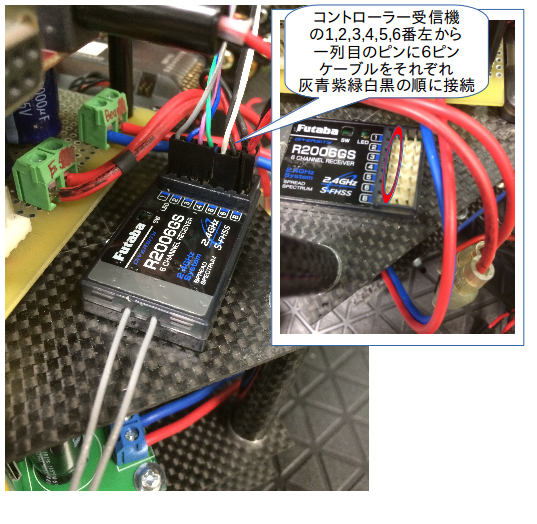
\includegraphics[width=140mm]{img/setuzoku3.png}
\end{center}
\caption{APMとコントローラ受信機への接続1}
\label{fig:setuzoku3}
\end{figure}

もう片方をAPM本体INPUTS端子上から図\ref{fig:setuzoku4}のように1段目1,2,3,4,5,6番ピンに緑青紫灰白黒の順に接続する.\\

\begin{figure}[H]
\begin{center}
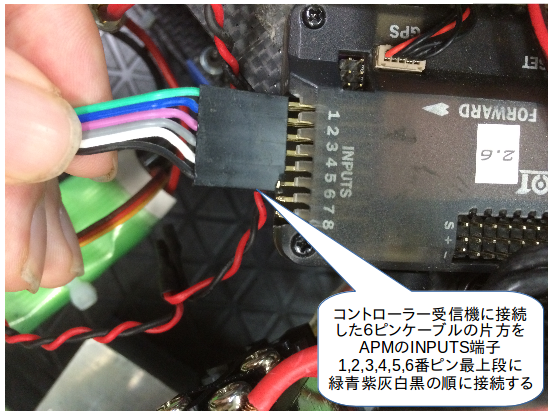
\includegraphics[width=140mm]{img/setuzoku4.png}
\end{center}
\caption{APMとコントローラ受信機への接続1}
\label{fig:setuzoku4}
\end{figure}

2)モータの接続\\
  X型Quad Rotorの各種プロペラモータの番号は図\ref{fig:setuzoku4}のよう  になっている.番号を把握した上で正しくAPMに接続しないと操縦した時,意図し  ない方向に機体が飛んでしまうので特に気をつけたい.

\begin{figure}[H]
\begin{center}
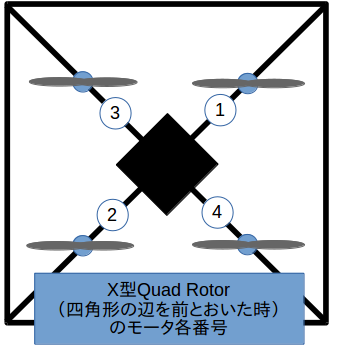
\includegraphics[width=110mm]{img/setuzoku5.png}
\end{center}
\caption{機体の各モータ番号}
\label{fig:setuzoku5}
\end{figure}

図\ref{fig:setuzoku5}を参照し,図\ref{fig:setuzoku6}のようにAPM本体OUTPUTS側に上から黄赤茶の順に,1番モータドライバのケーブルは1番ピン列に.2番モータドライバのケーブルは2番ピン列に,残り同様に4つのモータを接続する.

\begin{figure}[H]\cite{si2014}
\begin{center}
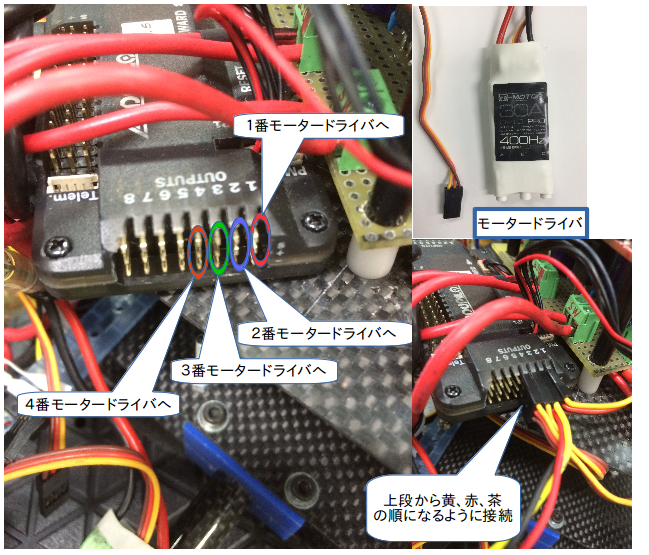
\includegraphics[width=140mm]{img/setuzoku6.png}
\end{center}
\caption{モータドライバとAPMの接続}
\label{fig:setuzoku6}
\end{figure}

APMとモータドライバを接続したあと,4つのモータのケーブルをモータドライバに図\ref{fig:setuzoku7}のように接続する.起動させた時,プロペラの回転方向が逆の場合左右のプラグを入れ替えると良い.

\begin{figure}[H]
\begin{center}
\includegraphics[width=140mm]{img/setuzoku7.png}
\end{center}
\caption{モータドライバとモータの接続}
\label{fig:setuzoku7}
\end{figure}

3)測域センサ(UTM-30LX)の接続\\
  センサ本体から伸びている4ピンコードとUSBケーブルを図\ref   {fig:setuzoku8}  のように接続していく.\\

\begin{figure}[H]
\begin{center}
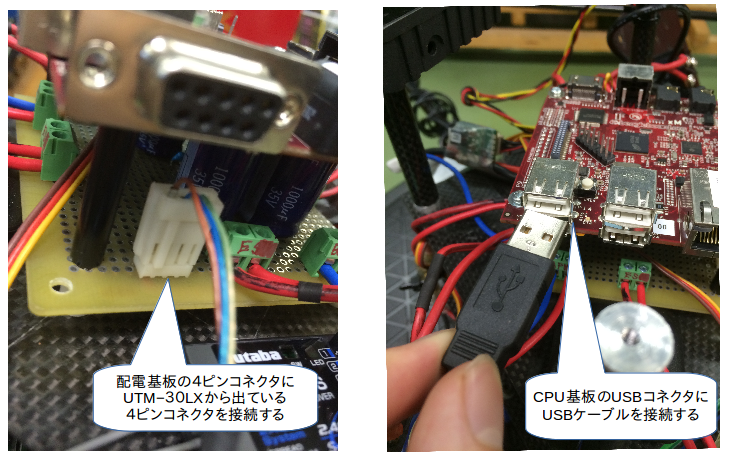
\includegraphics[width=140mm]{img/setuzoku8.png}
\end{center}
\caption{測域センサの接続}
\label{fig:setuzoku8}
\end{figure}

4)高度センサの接続\\
  図\ref{fig:setuzoku9}のように,APM本体のTelem.と書かれた端子横のA0端 子に図のような色の配列で接続する.\\

\begin{figure}[H]
\begin{center}
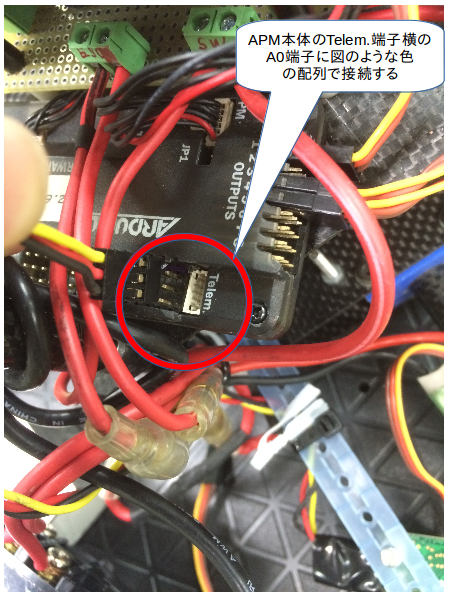
\includegraphics[width=100mm]{img/setuzoku9.png}
\end{center}
\caption{高度センサの接続}
\label{fig:setuzoku9}
\end{figure}

5)GPSセンサ(3DR)の接続\\
 図\ref{fig:setuzoku10}のように3DRから伸びているコードを接続する.

\begin{figure}[H]
\begin{center}
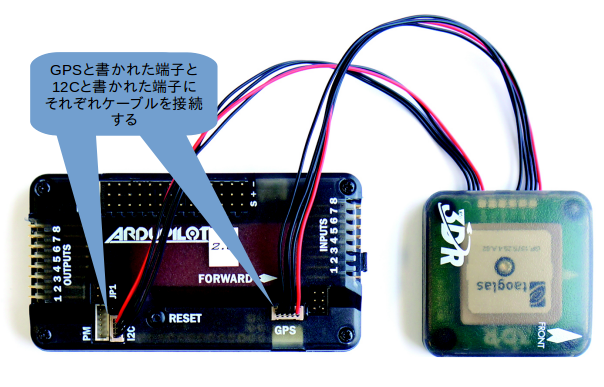
\includegraphics[width=140mm]{img/setuzoku10.png}
\end{center}
\caption{GPSセンサの接続}
\label{fig:setuzoku10}
\end{figure}

6)システムの全体図を示す.\\
 図\ref{fig:haisenzu2}に配線図を示す.\\
 図\ref{fig:haisenzu1}にビーグルボードと他の基板との接続図を示す.\\

\begin{figure}[H]
\begin{center}
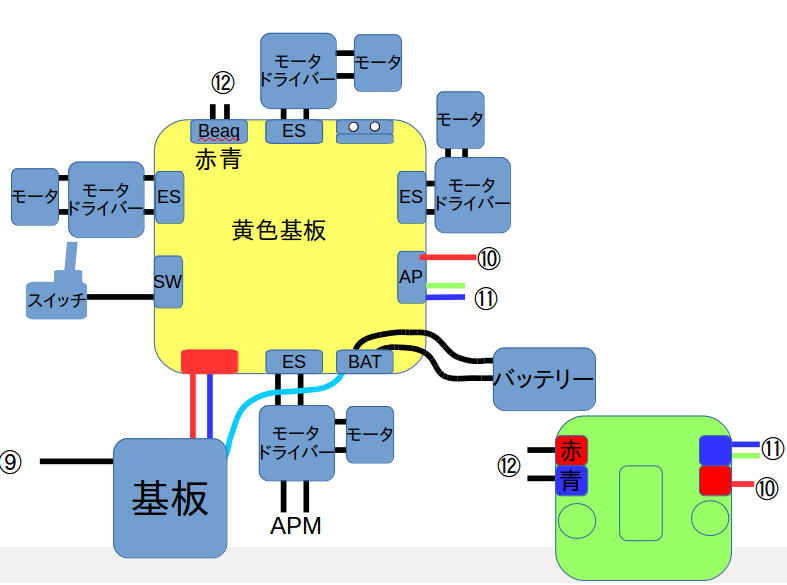
\includegraphics[width=100mm]{img/haisenzu2.png}
\end{center}
\caption{配線基板}
\label{fig:haisenzu2}
\end{figure}

\begin{figure}[H]
\begin{center}
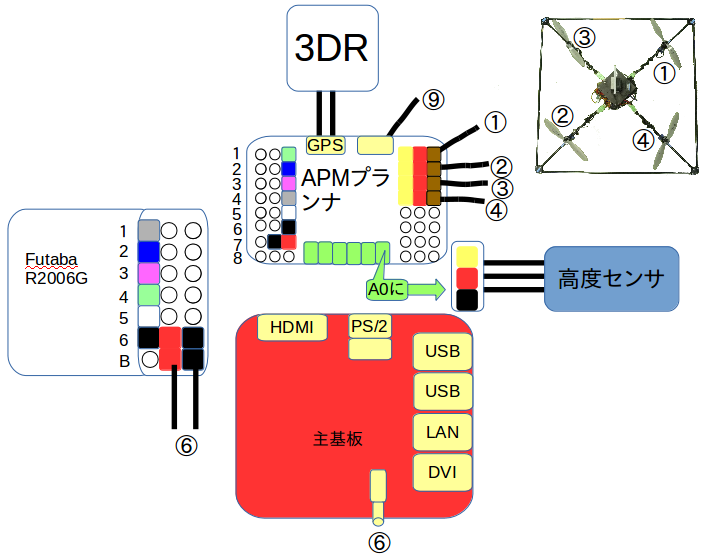
\includegraphics[width=100mm]{img/haisenzu1.png}
\end{center}
\caption{ビーグルボード}
\label{fig:haisenzu1}
\end{figure}


\section{Quad Rotorの移動方法}
上昇,下降は全てのモータの回転数を調節することにより行う.前後左右に移動する場合は進行方向と反対のモータ2つの回転数を上げることにより機体自体が,進行方向に傾き進む.

\begin{figure}[H]
\begin{center}
\includegraphics[width=100mm]{img/kaitennhouhou1.png}
\end{center}
\caption{UAVの基本動作}
\label{fig:kaitennhouhou1}
\end{figure}

回転方法は対角のモータの回転数を調節して行う.Quad Rotorのプロペラは対角で同じ方向に回転していて,回転したい方向と反対に回転しているモータの回転数を上げることにより反動トルクが生まれ機体が回転する.

\begin{figure}[H]
\begin{center}
\includegraphics[width=90mm]{img/kaiten.png}
\end{center}
\caption{反動トルクを利用したヨー回転}
\label{fig:kaiten}
\end{figure}

\begin{figure}[H]
\begin{center}
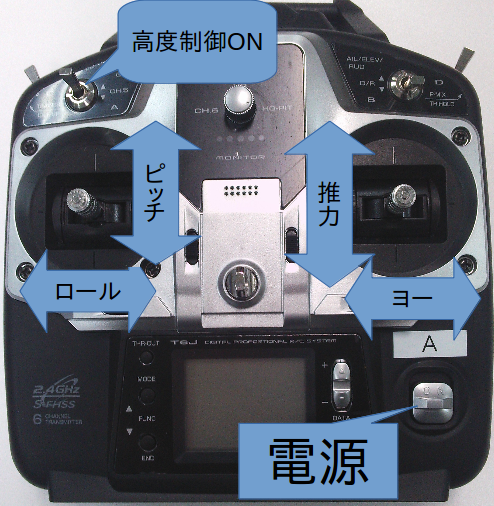
\includegraphics[width=90mm]{img/sousa.png}
\end{center}
\caption{コントローラーの操作}
\label{fig:7}
\end{figure}


\section{想定する障害物の避け方}

\begin{figure}[H]
\begin{center}
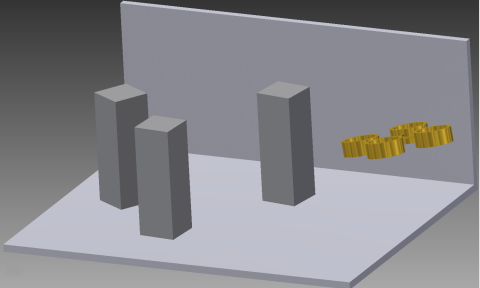
\includegraphics[width=80mm]{img/3.png}
\end{center}
\caption{障害物を避けるUAV}
\label{fig:3}
\end{figure}

UAVには一軸レーザ距離センサを搭載するので,図\ref{fig:3}に示す様に両側の壁と進行方向にあると思われる障害物の認識をセンサで読み取りながら進んでく.通常のスキャン式レーザ距離計であれば周辺状況を瞬時に取得可能であるが\cite{suzuki2011}\cite{kumada2010},一軸レーザ距離計では不可能であるので以下の壁沿い飛行方式を考えている.\\
(1)壁と進行方向にある障害物をセンサで読み取りながら進む.


\begin{figure}[H]
\begin{center}
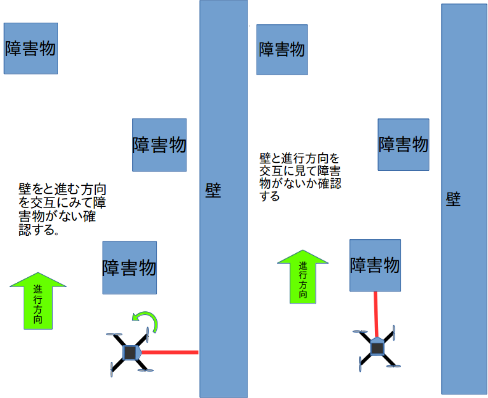
\includegraphics[width=80mm]{img/4.png}
\end{center}
%\caption{(1)周辺の状況を確認}
\label{fig:4}
\end{figure}

(2)障害物を発見できたならば,障害物を回避するために障害物をセンサで認識し横方向に進行する.


(3)障害物と機体の大きさ分の移動を終えたならば,壁方向を向き機体分移動する.


\begin{figure}[H]
\begin{center}
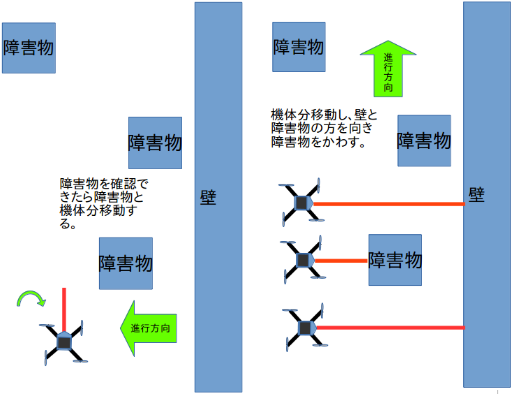
\includegraphics[width=80mm]{img/5.png}
\end{center}
%\caption{(2),(3)障害物を避ける}
\label{fig:5}
\end{figure}

(4)機体と障害物が並ぶ時,障害物をセンサで認識と進行方向に障害物が確認できるかを認識しながら障害物をかわす.


\begin{figure}[H]
\begin{center}
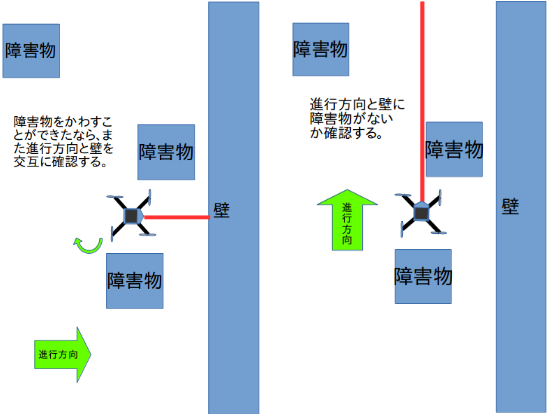
\includegraphics[width=80mm]{img/6.png}
\end{center}
\caption{壁沿い飛行の構想}
\label{fig:6}
\end{figure}

以上のような動作を続けることができれば,障害物に接触することなく室内全体のおおよその地形を読み取ることができるのではないかと思われる。

\chapter{周辺状況の取得実験}本実験は改良,軽量化をおこなった一軸レーザセンサが正しく動作し,実際に使用するにあたり問題なく周囲の状況を正しく読み取ることができるかを検証するものである.

\section{実験装置}
 1)ターンテーブル\\
  図\ref{fig:te-buru}に示す,ターンテーブルはUAV固定することで飛行時の高度  の固定と,四枚のプロペラの力で回転を行わせる.\\
   2)自作UAV\\
  図\ref{fig:UAV}に示す,実際のUAVの回転速度を再現するために使用する.\\
   3)プロポ\\
  図\ref{fig:puropo}に示すUAVの操縦を行うためのコントローラー.\\
   4)安定化電源\\
  図\ref{fig:dengen}に示す,安定した電力を供給が可能なので正確なデータの収  集が見込める.\\
   5)ノートパソコンを\\
  図\ref{fig:PC}に示す,センサで測定したデータを受け取るため.\\
   6)改良したセンサ\\
  図\ref{fig:sensakai}に示す,データを収集.\\
   7)無線ルーター\\
  図\ref{fig:rutor}に示す,パソコンのデータの送受信.\\


\begin{figure}[H]
\begin{center}
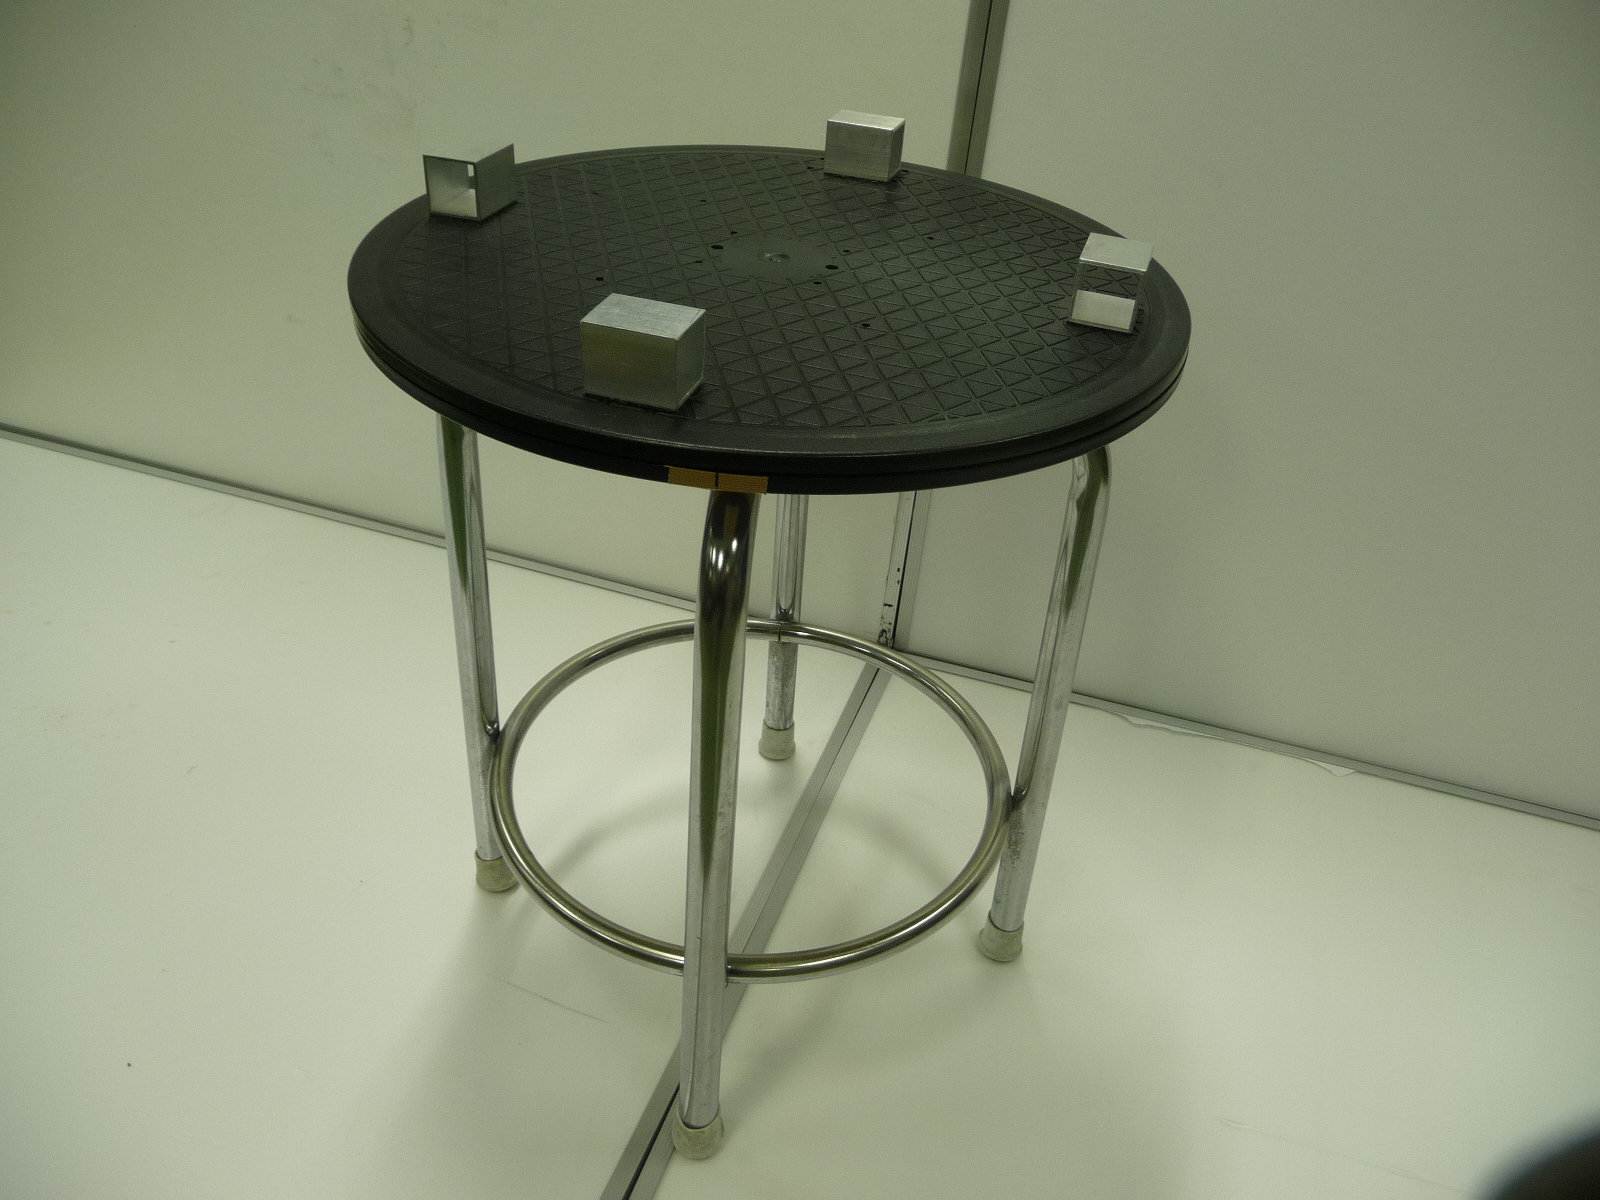
\includegraphics[width=80mm]{img/te-buru.jpg}
\end{center}
\caption{ターンテーブル}
\label{fig:te-buru}
\end{figure}

\begin{figure}[H]
\begin{center}
\includegraphics[width=80mm]{img/UAV.jpg}
\end{center}
\caption{自作UAV}
\label{fig:UAV}
\end{figure}

\begin{figure}[H]
\begin{center}
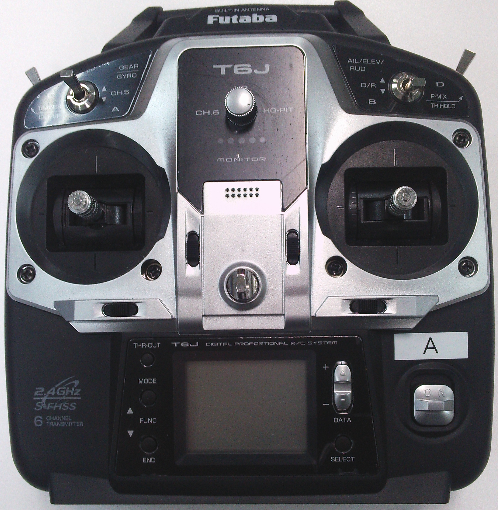
\includegraphics[width=80mm]{img/puropo.png}
\end{center}
\caption{プロポ}
\label{fig:puropo}
\end{figure}

\begin{figure}[H]
\begin{center}
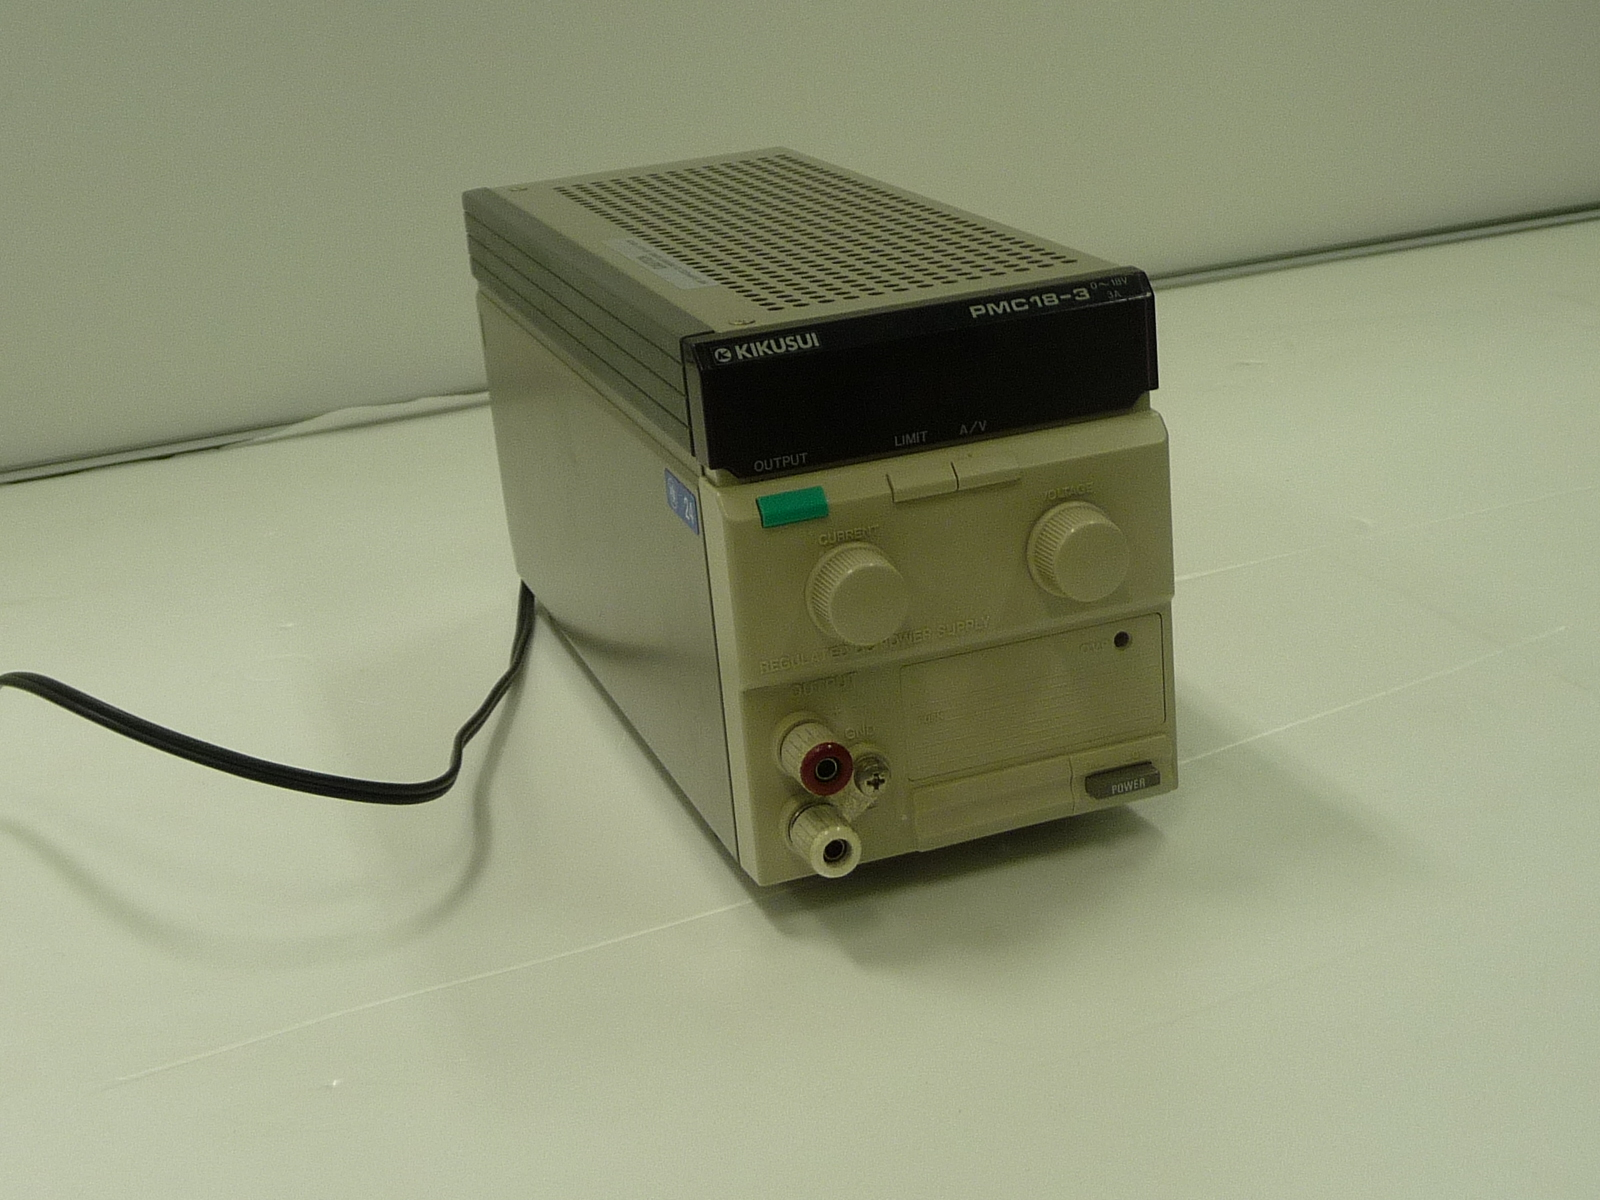
\includegraphics[width=80mm]{img/dengen.jpg}
\end{center}
\caption{電源}
\label{fig:dengen}
\end{figure}

\begin{figure}[H]
\begin{center}
\includegraphics[width=80mm]{img/PC.jpg}
\end{center}
\caption{ノートパソコン}
\label{fig:PC}
\end{figure}

\begin{figure}[H]
\begin{center}
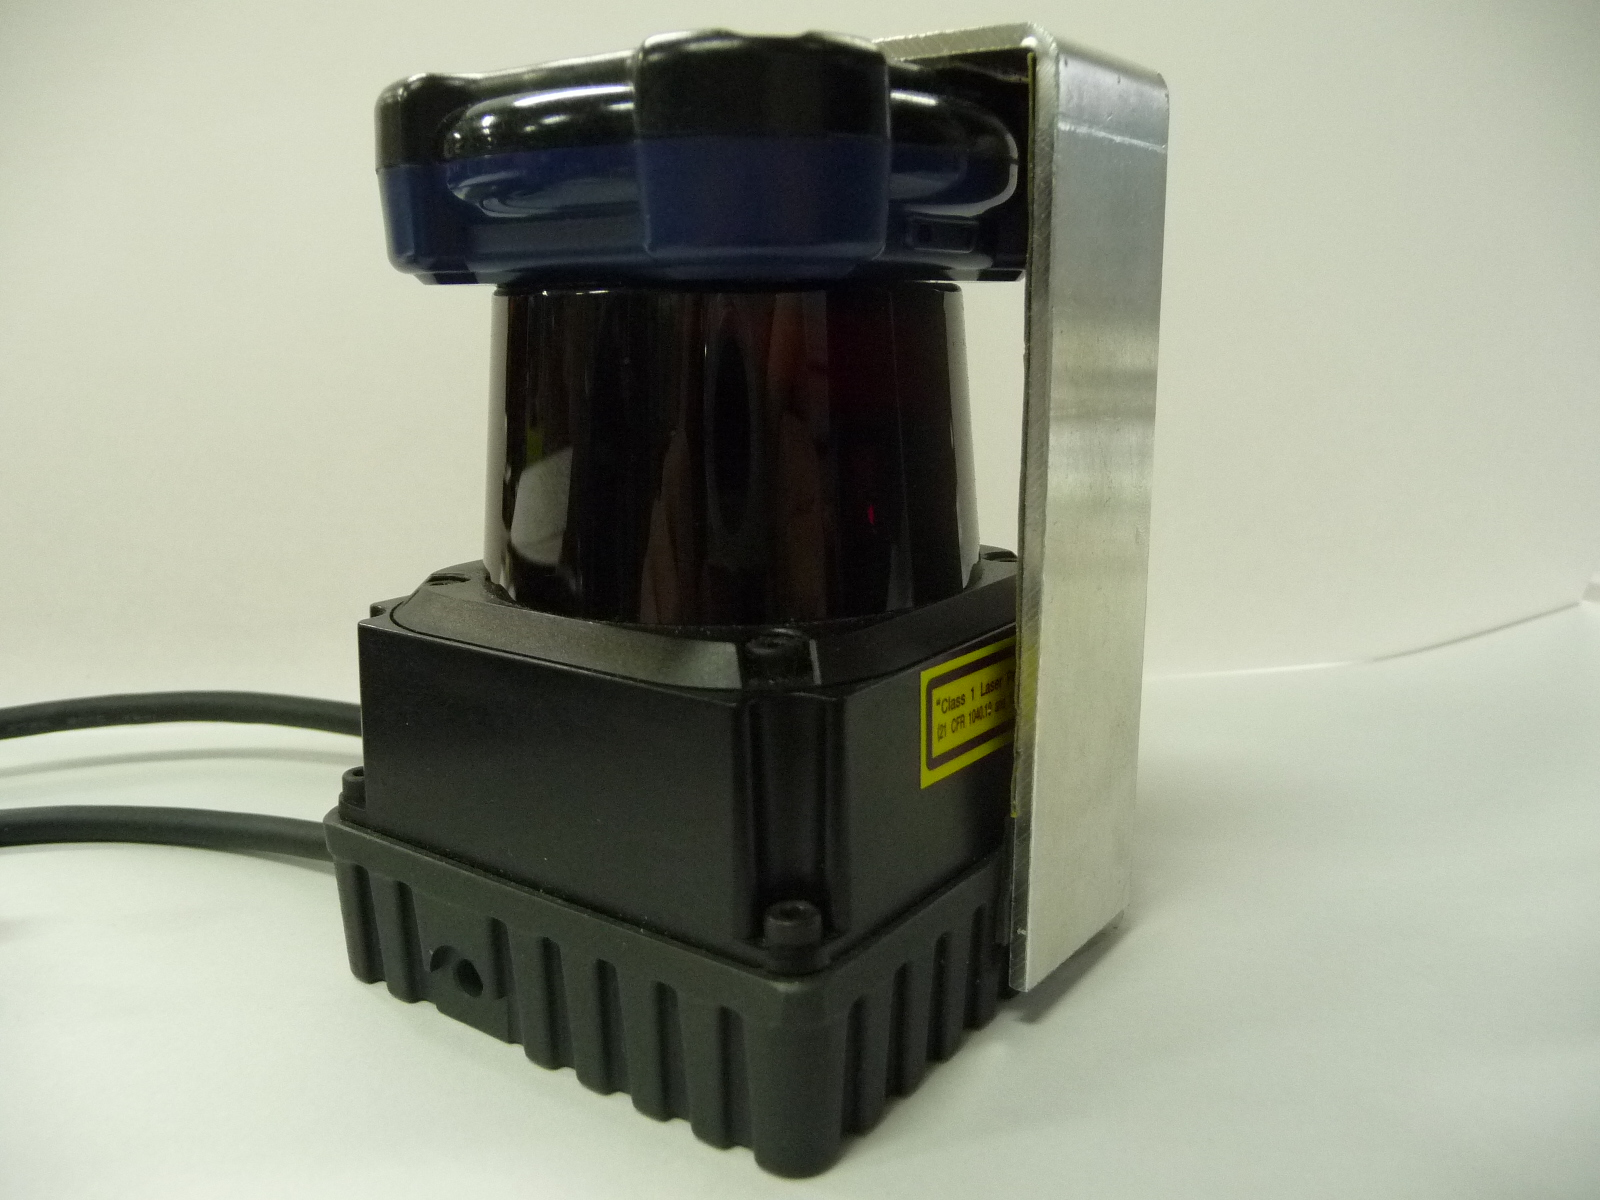
\includegraphics[width=80mm]{img/sensakai.jpg}
\end{center}
\caption{改良したセンサ}
\label{fig:sensakai}
\end{figure}

\begin{figure}[H]
\begin{center}
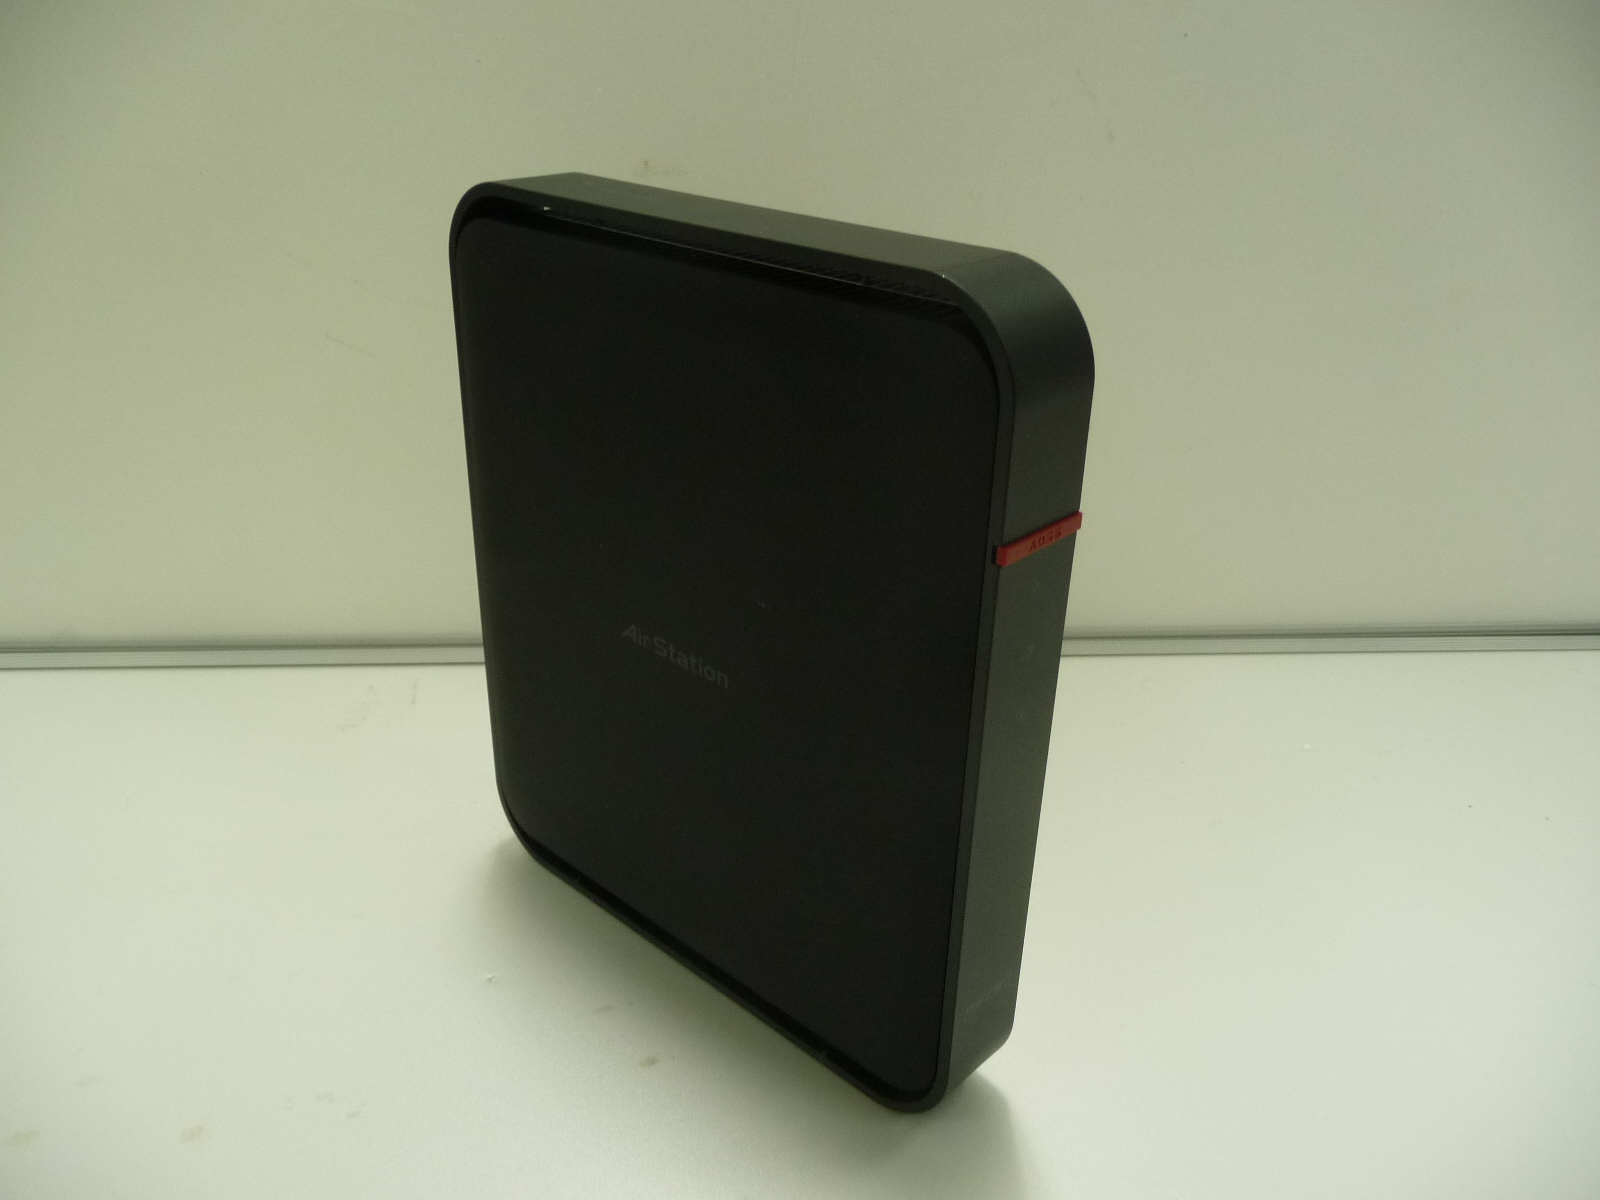
\includegraphics[width=80mm]{img/rutor.jpg}
\end{center}
\caption{無線ルーター}
\label{fig:rutor}
\end{figure}

図\ref{fig:tizu2}にスキャン式センサを用いて地図作成する場合に使用する実験装置の構成図を示す.
図\ref{fig:rutor}にターンテーブルと実際に飛行させ実験を行う場合に使用する実験装置の構成図を示す

\begin{figure}[H]
\begin{center}
\includegraphics[width=80mm]{img/tizu2.png}
\end{center}
\caption{スキャン式センサ実験の構成}
\label{fig:tizu2}
\end{figure}

\begin{figure}[H]
\begin{center}
\includegraphics[width=80mm]{img/Wifi.png}
\end{center}
\caption{ターンテーブル・飛行実験の構成}
\label{fig:Wifi}
\end{figure}



\section{実験方法}図\ref{fig:8}にスキャン式センサで取得した地図を示す.\\

\begin{figure}[H]
\begin{center}
\includegraphics[width=100mm]{img/8.png}
\end{center}
\caption{取得環境の簡易地図}
\label{fig:8}
\end{figure}

\subsection{ターンテーブルでの実験}UAVを図\ref{fig:7}のようにターンテーブルの上に固定する.校舎前でプロポを使用し,UAVを水平回転させ,周辺の地形読み取りを行い地形を正しく認識できるかを検証する.\\
 
\subsection{飛行実験}ターンテーブルの実験同様に校舎前で実験を行う,UAVを実際に飛行させ一定の高度に保ちその場で水平回転させ,周辺の地形を正しく読み取れるか検証する.実験は2箇所で行う.

\begin{figure}[H]
\begin{center}
\includegraphics[width=120mm]{img/7.png}
\end{center}
\caption{UAVの固定方法}
\label{fig:7}
\end{figure}



\section{実験結果}
\subsection{ターンテーブルでの実験結果}固定台に固定し実験の結果を図\ref{fig:9}に示す.実線で描かれた部分が壁であり,連続した丸印がレーザが壁と認識した箇所である.
多少の差異は見られるものの,大きくずれてしまったところは見られなかった.自動制御を行い飛行するには十分な精度があると見られる.

\begin{figure}[H]
\begin{center}
\includegraphics[width=120mm]{img/9.png}
\end{center}
\caption{ターンテーブルでの実験結果}
\label{fig:9}
\end{figure}

\subsection{飛行実験結果}飛行実験ではUAVがアンバランスなせいか旋回中に移動してしまい,地図と一致するデータの取得は難しいが,図\ref{fig:034}と図\ref{fig:035}に示すように一部を地図と一致させUAV
の位置を調べることができる.

\begin{figure}[H]
\begin{center}
\includegraphics[width=150mm]{img/034.png}
\end{center}
\caption{飛行実験結果1}
\label{fig:034}
\end{figure}

\begin{figure}[H]
\begin{center}
\includegraphics[width=150mm]{img/035.png}
\end{center}
\caption{飛行実験結果2}
\label{fig:035}
\end{figure}

\section{考察}
ターンテーブルの実験では,2次元の地図とおおむね一致したので実験は成功した.
手動でUAVを飛行させた実験は、UAVが一定の位置で回転を行うのが困難なので,地図に誤差が生じた.
しかし,データの中かで特徴がはっきりした所と地図を一致させる事でUAVの位置を調べることができる.



\chapter{結言}
\section{本研究のまとめ}小型UAVに搭載する軽量化した一軸レーザー距離センサを用いた壁沿い飛行を行う機体の実現にあたり,一軸センサでの周辺状況の取得についての実験により有効性を確認した.
一軸センサの特性上,センサ正面の距離を測定することしかできず,左右の障害物を特定するためには実際に機体がそちらの方向を向き,計測しながら移動する必要があった.
そこで前方の壁の距離を測り,移動したい方向に一度センサを機体ごと向け,障害物がないかを調べながら徐々に移動することで,周辺状況の計測することを考えた.そのため,機体をゆっくり回転させて周辺状況を取得する実験を試みたが,実験の結果一軸レーザーセンサによる周辺状況の取得は成功した.機体がずれる場合は特徴のある箇所と地図を重ねる事ができれば,機体の位置を作成された地図から調べる事ができる.

\section{今後の課題}災害現場などで活躍するにはより複雑な地形を読み取り対応する必要がある.今後は実際に飛行プログラムと連携し,取得したデータを用いながら移動する手法の検討に入る予定である.


\begin{thebibliography}{8}
\bibitem{hirokawa2007}廣川類,久保大輔,鈴木真二,辰己薫,實松洋平,大畠龍介.(2007).小型無人機用自律誘導システムの設計と評価.自動制御連合講演会講演論文集,50(0),87-87.\\
\bibitem{sibata2003}柴田英貴.(2003).UAV(Unmanned Aerial Vehicle)と画像処理.情報処理学会研究報告.CVIM,[コンピュータビジョンとイメージメディア],2003(2),31-36.\\
\bibitem{suzuki2011}鈴木太郎,橋詰匠,鈴木真二.(2011).小型自律飛行ロボット(UAV)の活用による簡便な地物計測.建設の施工企画,(740),65-69.\\
\bibitem{kumada2010}熊田貴之,宇多高明,鈴木真二,酒井和也,野志保仁,森田学,柄沢研治.(2010).無人飛行機(UAV)による新しい海岸モニタリング手法,海洋開発論文集,第26巻.\\
\bibitem{si2014}織田隆誠,木村俊介,村田涼真:“1軸レーザ距離センサを用いたQuad Rotorの周辺認識についての研究”.東京ビックサイト,2014年12月17日,公益社団法人計測自動制御学会システムインテグレーション部門.2014年12月17日.
\end{thebibliography}

\chapter*{謝辞}
\addcontentsline{toc}{chapter}{謝辞}
本論文作成にあたりテーマの決定,研究の考え方,方法のまとめ方など全てにおいて長期にわたって厳しくも熱意のあるご指導,ご鞭撻していただいた,伊藤恒平教授に厚く御礼申し上げます.


特に分析においても論文の書き方においても論文を何度も読んでいただき,指導していただいた伊藤恒平教授に大変ご苦労をかけてしまいましたことにも心よりお詫び申し上げたいです.


同級生のメンバーには論文の作成,修正にご協力いただき心より感謝しております.
その他、助けていただいた多くの皆様に心から感謝しております.ありがとうございました.

\end{document}

